\documentclass[11pt]{article}
\usepackage{amsmath}
\usepackage{geometry}                % See geometry.pdf to learn the layout options. There are lots.
\geometry{letterpaper}                   % ... or a4paper or a5paper or ... 
%\geometry{landscape}                % Activate for for rotated page geometry
%\usepackage[parfill]{parskip}    % Activate to begin paragraphs with an empty line rather than an indent
\usepackage{graphicx}
\usepackage{fullpage}
\usepackage{amssymb}
\usepackage{epstopdf}
\usepackage{url}
\DeclareGraphicsRule{.tif}{png}{.png}{`convert #1 `dirname #1`/`basename #1 .tif`.png}
\date{}
\title{Homework 1}
\author{(Inference and Representation) 
\\ Due September 16 on NYU Classes.  }
%\date{}                                           % Activate to display a given date or no date

\begin{document}
\maketitle
 
 Problems 1 and 2 are from Murphy, chapter 2. Problems 3 and 4 are from Joan Bruna's course.
\begin{enumerate}
\item  Probabilities are sensitive to the form of the question that was used to generate the answer. My neighbor has two children. Assuming that the gender of a child is like a coin flip, it is most likely, a priori, that my neighbor has one boy and one girl, with probability 1/2. The other possibilities—two boys or two girls—have probabilities 1/4 and 1/4.

\begin{enumerate}
\item Suppose I ask him whether he has any boys, and he says yes. What is the probability that one child is a girl?
\item Suppose instead that I happen to see one of his children run by, and it is a boy. What is the probability that the other child is a girl?
\end{enumerate}
\item Legal reasoning. Suppose a crime has been committed. Blood is found at the scene for which there is
no innocent explanation. It is of a type which is present in 1\% of the population.
\begin{enumerate}
\item The prosecutor claims: “There is a 1\% chance that the defendant would have the crime blood type if he were innocent. Thus there is a 99\% chance that he guilty”. This is known as the prosecutor’s fallacy. What is wrong with this argument?
\item The defender claims: “The crime occurred in a city of 800,000 people. The blood type would be found in approximately 8000 people. The evidence has provided a probability of just 1 in 8000 that the defendant is guilty, and thus has no relevance.” This is known as the defender’s fallacy. What is wrong with this argument?
\end{enumerate}

\item \textbf{Hidden Markov models}. Harry lives a simple life. Some days he is Angry and some days he is Happy. But he hides his emotional state, and so all we can observe is whether he smiles, frowns, laughs, or yells. Harry’s best friend is utterly confused about whether Harry is actually happy or angry and decides to model his emotional state using a hidden Markov model.
Let $X_d \in \{\text{Happy, Angry}\}$ denote Harry’s emotional state on day $d$, and let $Y_d\in \{ \text{smile, frown, laugh, yell}\}$ denote the observation made about Harry on day $d$. Assume that on day 1 Harry is in the Happy state, i.e. $X_1 = $Happy. Furthermore, assume that Harry transitions between states exactly once per day (staying in the same state is an option) according to the following distribution: 

$p(X_{d+1} = \text{Happy} | X_d = \text{Angry}) = 0.1$, 

$p(X_{d+1} = \text{Angry} | X_d = \text{Happy}) = 0.1$, 

$p(X_{d+1} = \text{Angry} | X_d =\text{Angry}) = 0.9$, and 

$p(X_{d+1} = \text{Happy} | X_d = \text{Happy}) = 0.9$.

\noindent The observation distribution for Harry’s Happy state is given by 

$p(Y_d = \text{smile} | Xd = \text{Happy}) = 0.6$, 

$p(Y_d = \text{frown} | Xd = \text{Happy}) = 0.1$,  

$p(Y_d = \text{laugh} | Xd = \text{Happy}) = 0.2$,  and 

$p(Y_d = \text{yell} | Xd = \text{Happy}) = 0.1$. 

\noindent The observation distribution for Harry’s Angry state is 

$p(Yd = \text{smile} | Xd = \text{Angry}) = 0.1$, 

$p(Yd =\text{frown} | Xd = \text{Angry}) = 0.6$, 

$p(Yd = laugh | Xd =\text{Angry})=0.1,$ and 

$p(Yd =\text{yell} | Xd =\text{Angry})=0.2.$

\noindent All of this is summarized in the following figure:

\begin{center}
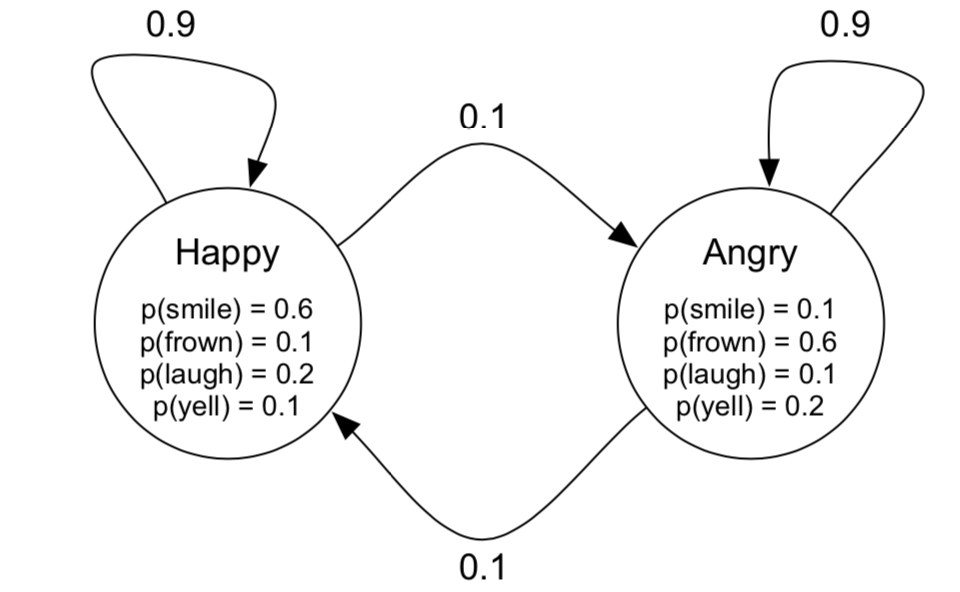
\includegraphics[width=0.7\textwidth]{figure}
\end{center}

\begin{enumerate}
\item What is $p(X_2 = \text{Happy})$?
\item What is $p(Y_2 = \text{frown})$?
\item What is $p(X_2 = \text{Happy} | Y2 = \text{frown})$?
\item What is $p(Y_{60} = \text{yell})$?
\item Assume that $Y_1 =Y_2 =Y_3 =Y_4 =Y_5 =\text{frown}$. What is the most likely sequence of the states? That is, compute the MAP assignment $$\arg \max_{x1,\ldots,x5} p(X_1 = x_1,...,X_5 =x_5 |Y_1 =Y_2 =Y_3 =Y_4 =Y_5 =\text{frown})$$
\end{enumerate}

\item \textbf{Naive Bayes classifier}
\begin{enumerate}
\item The dataset we will be using is a subset of 2005 TREC Public Spam Corpus, containing 9000 training examples and 1000 test examples. You can download it here 

\url{https://courses.cs.washington.edu/courses/csep546/12sp/psetwww/3/NDA.htm}

Each line in the train/test files represents a single email with the following space-delimited properties: the first is the email ID (in the form /xxx/yyy), the second is whether it is ‘\emph{spam}’ or ‘\emph{ham}’ (non-spam), and the rest are words followed by their occurrence numbers. (Note that numbers may be words, so don’t worry if a line contains multiple numbers in a row). The data has been pre-processed to remove non-word characters (e.g. ‘!’) and to select features similar to what Mehran Sahami did in his original paper \url{http://robotics.stanford.edu/users/sahami/papers-dir/spam.pdf}
though with larger cut-offs since our corpus is larger.

\item Using the training data, compute the prior probabilities $P(spam)$ and $P(ham)$. What
is $P(spam)$?
\item Determine the vocabulary and compute the conditional probabilities $P(w_i |spam)$ and $P(w_i |ham)$.

In this context, it is possible that none of emails labeled as say spam contain a
particular word $w_j$ . Then $P(w_j |spam) = 0$ and $P(spam) \pi_i P (w_i |spam) = 0$. To
address this use a so-called $m$-estimate given by $P(w_j|spam) = \frac{n_c+mp}{n+m}$ where
\begin{itemize}
\item $n$ is the number of training examples which are spam
\item $n_c$ is the number of examples, which are spam and which contain $w_j$
\item $p$ is prior estimate for $P(w_i |spam)$, e.g., $p = 1/|Vocabulary|$)
\item $m$ is weight given to the prior, i.e., number of deemed training examples, e.g.,
$m = |Vocabulary|$.
\end{itemize}
In this context we consider each word as a training example, so $n$ is the total number of words (in either ham or spam documents) and $n_c$ is the number of times $w_j$ appeared in those documents (including multiple occurrences in the same email).

What are the 5 most likely words given that a document is spam? What are the 5 most likely words given that a document is ham?

\item  Use these probabilities to classify the test data and report the accuracy (i.e. the percentage of correct classifications). Note that directly computing $P(spam|w_1,\ldots,w_n)$ and $P(ham|w_1,...,w_n)$ can cause numerical precision issues, since the unnormalized probabilities are very small (i.e. the numerator in Bayes’ theorem). Instead, you should compare the log-probabilities of being ham/spam.
\item Vary the m parameter, using $m = |Vocabulary| \times [1, 10, 100, 1000, 10000]$ and plot the accuracies vs. $m$. What assumptions are we making when the value of $m$ is very large vs. very small? How does this affect the test accuracy?
\item  If you were a spammer, how would you modify your emails to beat the classifiers we have learned above?

With your answers, please include your Python code and a report containing: 
\begin{itemize}
\item A high-level description on how your code works.
\item The accuracies you obtain.
\item If all your accuracies are low, tell us what you have tried to improve and what you suspect is failing.
\end{itemize}

\end{enumerate}
\end{enumerate}
\end{document}  